As we have seen in the preceding chapters there is quite a large range of models designed to generate data such as images, audio or video. Despite this high diversity only some of them – in particular GANs and VAEs – achieved outstanding success \cite{biggan, vqvae2}, on the basis of which they were heavily improved in the last years. It is therefore quite difficult to come up with a new model that is able to quickly keep up with these highly adapted models. The fact that in this harsh environment \textit{Score-Based Generative Models} \cite{score_1, score_3, score_2} were able to achieve state-of-the-art results explains why they recently gained a lot of attention and makes them a new promising contender to the field of well established generative models.

As Score-Based Generative Models were going through a lot of changes since the first publication, the next sections chronologically explain Score-Based Generative Models and their evolution in detail. In \hyperref[sec:4.1]{Sec.\,4.1} a brief overview of the core concepts of Score-Based Generative Models is given, followed by \hyperref[sec:4.2]{Sec.\,4.2} explaining why these core concept fails when being used without adaptions. \hyperref[sec:4.3]{Sec.\,4.3} then presents how adding noise of discrete noise scales to the data distribution makes Score-Based Generative Modeling feasible, after which \hyperref[sec:4.4]{Sec.\,4.4} generalizes this concept by introducing continuous noise governed by a Stochastical Differential Equation (SDE). Finally in \hyperref[sec:4.5]{Sec.\,4.5} the theory behind controllable generation is presented.

%%%%%%%%%%%%%%%%%%%%%%%%%%%%%%%%%%%%%%%%%%%%%%%%%%%%%%%%%%%%%%%%%%%%%%%%%%%%%%%%%%%%%%%%%%%%%%%%
\section{The idea behind Score-Based Generative Models} \label{sec:4.1}
\sectionmark{The idea behind SGM}
In general the most basic Score-Based Generative Model consists of two core ideas: First, estimating the score $\nabla_{\vec{x}}\log p(\vec{x})$ of an unknown data distribution $p_{data}(\vec{x})$ of a dataset $\{\vec{x}_i\in \mathbb{R}^d\}_{i=1}^N$ of $n$ i.i.d samples. This process is referred to as \textit{Score Matching} \cite{score_matching_original}. And second, using \textit{Langevin Dynamics} \cite{langevin1, langevin2} to sample from the data distribution by starting with an initial value $\tilde{\vec{x}_0}$ from a prior distribution $\pi(\vec{x})$. This value is then gradually transformed by $T$ recursive steps of Langevin Dynamics and will finally come out as $\tilde{\vec{x}}_T$ where $p(\tilde{\vec{x}}_T)\approx p_{data}(\vec{x})$, which makes it a nearly perfect sample of $p_{data}(\vec{x})$. The resulting generative modeling framework is called \textit{Score Matching Langevin Dynamics} (SMLD).
%
\subsection{Score Matching} \label{sec:4.1.1}
This section gives an overview of Score Matching and how this technique can be used to get an objective for a score estimator, i.e. the model that is trained to estimate the score $\nabla_{\vec{x}}\log p_{data}(\vec{x})$ of the data distribution $p_{data}(\vec{x})$. The section is mathematically fairly intensive, and for that reason the main goal of this section is to provide a good feeling for why using the estimation of the score function as a model objective is a reasonable idea.

Score Matching \cite{score_matching_original} is a technique that originates from probabilistic models and their difficulties to be trained on an unnormalized probability density function $\tilde{p}(\vec{x})$ of a data distribution $p_{data}(\vec{x})$. The task of such a model $p_\theta(\vec{x})$ is to learn parameters $\theta$ such that $p_\theta(\vec{x})=p_{data}(\vec{x})$ where $p_{data}(\vec{x})$ is the normalized density function defined as
%
\begin{equation}
    p_{data}(\vec{x})=\frac{\tilde{p}(\vec{x})}{Z},\quad Z=\int\tilde{p}(\vec{x})d\vec{x}\,.
\end{equation}
%
$Z$ is called the partition function and can be understood as a normalization constant. It is this partition function $Z$ that causes the models difficulty to achieve its task. This is because the computation of $Z$ is intractable, meaning that it cannot be solved in polynomial time or rather its complexity is at least $\mathcal{O}(k^n)$, where $k>1$ is some constant and $n\in\mathbb{N}$ is the length of an input. The reason to use the score function to overcome this problem can be easily seen by using the calculation rules for logarithms to get $\log p(\vec{x})=\log\tilde{p}(\vec{x})-\log Z$. It is therefore obvious that the score function $\nabla_{\vec{x}}\log p(\vec{x})$ does not depend on the intractable partition function $Z$.

Score Matching uses this fact by minimizing the Fisher divergence between $p_{data}(\vec{x})$ and $p_\theta(\vec{x})$, which is defined as
%
\begin{equation} \label{equ:4.2}
    L(\theta)\triangleq\frac{1}{2}\mathbb{E}_{p_{data}}[\norm{s_\theta(\vec{x})-\nabla_{\vec{x}}\log p_{data}(\vec{x})}^2_2],
\end{equation}
%
where $s_\theta(\vec{x})\triangleq\nabla_{\vec{x}}\log p_\theta(\vec{x})$ and $\norm{\cdot}_2$ is the euclidean norm. From here on we now begin to transition from the probabilistic model $p_\theta(\vec{x})$ to the score model $s_\theta(\vec{x})$. \hyperref[equ:4.2]{Equ.\,4.2} is the formulation of Score Matching which can be used in an integrated form as part of the model objective for probabilistic models. But beyond that Score Matching can also be used as a standalone model objective for the so called \textit{Score-Based Models}.

Ultimately, both probabilistic models and score-based models learn the data distribution so that it is possible to generate samples from it. However probabilistic models aim to learn the data distribution itself. Score-based models ($s_\theta(\vec{x})$) aim to learn the score of the data distribution. In order to train a score-based model we have to reformulate the objective in \hyperref[equ:4.2]{Equ.\,4.2} as it is still not readily usable for leaning score-models because the data distribution $p_{data}(\vec{x})$ is typically unknown and so is $\nabla_{\vec{x}}\log p_{data}(\vec{x})$. 

To address the problem of the unknown data distribution \textit{Denoising Score Matching} \cite{denoise_score} was proposed. Denoising Score Matching introduces noise to \hyperref[equ:4.2]{Equ.\,4.2} so that $\nabla_{\vec{x}}$ does not operate directly on the unknown distribution. A noise distribution $q_\sigma(\tilde{\vec{x}}|\vec{x})$ is applied to the data distribution to get a perturbed data distribution $q_\sigma(\vec{x})=\int q_\sigma(\tilde{\vec{x}}|\vec{x})p_{data}(\vec{x})d\vec{x}$. When the noise is small ($q_\sigma(\vec{x})\approx p_{data}(\vec{x})$) then $s_\theta(\vec{x})=\nabla_{\vec{x}}\log q_\sigma(\vec{x})\approx\nabla_{\vec{x}}\log p_{data}(\vec{x})$ holds true. The objective of Denoising Score Matching follows as
%
\begin{equation} \label{equ:4.3}
    \theta^*=\underset{\theta}{\arg\min}\frac{1}{2}\mathbb{E}_{q_\sigma(\tilde{\vec{x}}|\vec{x})p_{data}(\vec{x})}[\norm{s_\theta(\vec{x})-\nabla_{\vec{x}}\log q_\sigma(\tilde{\vec{x}}|\vec{x})}^2_2].
\end{equation}
%
In conclusion \hyperref[equ:4.3]{Equ.\,4.3} is the training objective for score based models that is further used throughout this thesis. Nevertheless there are also other Score Matching techniques such as \textit{Sliced Score Matching} \cite{song2019sliced} that could be used, but it turns out that Denoising Score Matching is considerably faster. The objective of Score-Based Models (\hyperref[equ:4.2]{Equ.\,4.2}) has several desirable properties which makes it a reasonable approach for a generative model. As shown above the objective does not rely on the intractable partition function $Z$. Therefore the objective is almost always tractable which has the implications that there is no special model architecture necessary. Furthermore the objective can be optimized without adversarial training (\hyperref[sec:gans]{Sec.\,3.2}) making it easier and more stable to train.

\subsection{Langevin Dynamics} \label{sec:4.1.2}
As described in \hyperref[sec:4.1.1]{Sec.\,4.1.1} a score-model is tasked to estimate the score of the unknown data distribution $p_{data}(\vec{x})$ of a dataset. However the score of a distribution is not yet a generated image. Instead as it is the \textit{gradient} of the (log) data distribution it can be utilized to sample from $p_{data}(\vec{x})$ by transforming a value $\tilde{\vec{x}}_0$ of a prior distribution $\pi(\vec{x})$ to be part of the data distribution, following the gradient (the score) of the data distribution. There are some restrictions to what the prior distribution should look like but for the considerations of score-based models the prior distribution is just Gaussian noise, so $\pi(\vec{x})\sim\mathcal{N}(\vec{x}, \vec{0}, \vec{I})$.

The process used for sampling is based on \textit{Langevin Dynamics}, a concept from physics, that was adopted to machine learning \cite{langevin1, langevin2}. In Physics the \textit{Langevin Equation} describes particles moving in a potential which additionally are subject to random forces. This process is called \textit{Brownian Motion}. The Langevin equation reads as 
%
\begin{equation} \label{equ:4.4}
    \lambda \frac{\vec{x}(t)}{dt}=-\nabla V(\vec{x}(t))+\vec{\eta}(t),
\end{equation}
%
where $V$ is the potential the particle is moving in, $\vec{x}(t)$ is the particles position and $\vec{\eta}(t)$ is white noise. Commonly \hyperref[equ:4.4]{Equ.\,4.4} is written as an (Itô)-Stochastical Differential Equation (SDE)
%
\begin{equation} \label{equ:4.5}
    d\vec{x}(t)=\underbrace{-\nabla V(\vec{x}(t))\,dt}_\text{drift term}+\underbrace{\sqrt{2}\,d\vec{w}}_\text{diffusion term},
\end{equation}
%
with a drift term and a diffusion term. $\vec{w}$ denotes the \textit{Wiener Process} \cite{gardiner} which can be interpreted as the derivative of white noise. It is important to note that the positions of particles described by \hyperref[equ:4.5]{Equ.\,4.5} are distributed according to some probability density function $p(\vec{x})$ for all times $t\geq0$. This has some very useful consequences: We can choose the potential $V$ in such a way that the underlying probability density function is $p_{data}$. In this case we can sample from $p_{data}$.

To achieve the state where the positions particle described by the Langevin Equation are distributed by $p_{data}$ we have to choose $V(\vec{x})=-\log p_{data}({\vec{x}})$. Inserting $V(\vec{x})$ into \hyperref[equ:4.5]{Equ.\,4.5} results in
%
\begin{equation} \label{equ:4.6}
    d\vec{x}(t)=\nabla\log p_{data}(\vec{x})dt+\sqrt{2}\,d\vec{w}.
\end{equation}
%
Now the connection between Sampling with Langevin Dynamics and Score Matching (\hyperref[sec:4.1.1]{Sec.\,4.1.1}) can be seen. If the score of the data distribution is known we can sample from this distribution by using \hyperref[equ:4.6]{Equ.\,4.6}. For now $\vec{x}(t)$ was the position of a physical particle but \hyperref[equ:4.6]{Equ.\,4.6} is applicable for any $d$-dimensional data $\vec{x}(t)\in\mathbb{R}^d$, e.g. images. To use \hyperref[equ:4.6]{Equ.\,4.6} in the context of machine learning we cannot directly use the SDE as it describes continuous steps of infinitesimal size. We therefore discretize the SDE to discrete steps which can then be calculated by a computer. The resulting discretization in \hyperref[equ:4.7]{Equ.\,4.7} is called the Euler-Maruyama discretization of the SDE.
%
\begin{equation} \label{equ:4.7}
    \tilde{\vec{x}}_t=\tilde{\vec{x}}_{t-1}+\frac{\epsilon}{2}\nabla_{\vec{x}}\log p_{data}(\tilde{\vec{x}}_{t-1})+\sqrt{\epsilon}\,\vec{z}_t
\end{equation}
%
\hyperref[equ:4.7]{Equ.\,4.7} is a recursive algorithm that can be used to sample from $p_{data}$. Here $\tilde{\vec{x}}_0$ is a value from the prior distribution given above and the $\sim$ above the $\vec{x}$ shows that $\tilde{\vec{x}}$ is not in dataset nor described by the data distribution $p_{data}(\vec{x})$ but a random initial sample. Furthermore $z_t\sim\mathcal{N}(0, I)$ is Gaussian noise and $\epsilon$ is the step size of the algorithm. The sample after $T$ steps is a perfect sample of $p_{data}$ when $T\rightarrow\infty$ and $\epsilon\rightarrow0$. For application of this algorithm $T\gg0$ and $\epsilon\ll1$ are assumed.

Recapitulating what the algorithm does one can look at \hyperref[fig:4.1]{Fig.\,4.1}. The lines in the left image show a particle moving randomly according to \hyperref[equ:4.5]{Equ.\,4.5}. In the background the underlying (heart-shaped) data density function  is represented and in the right image samples are shown, where each of the dots is an initial sample from the prior distribution that was transformed using \hyperref[equ:4.7]{Equ.\,4.7}. When applying \hyperref[equ:4.7]{Equ.\,4.7} to infinite values from the prior distribution this process can be thought of as transforming one distribution to another one. As a side-note, the formulation of this integrated process is given by the \textit{Fokker-Planck-Equation} \cite{gardiner} – another important equation in physics. For the purposes of score-based models only a one-by-one application of \hyperref[equ:4.7]{Equ.\,4.7} is needed, essentially transforming one image from a noise distribution to an image that looks like it belongs the data distribution of the target dataset.
%
\begin{figure}[] \label{fig:4.1}
    \centering
    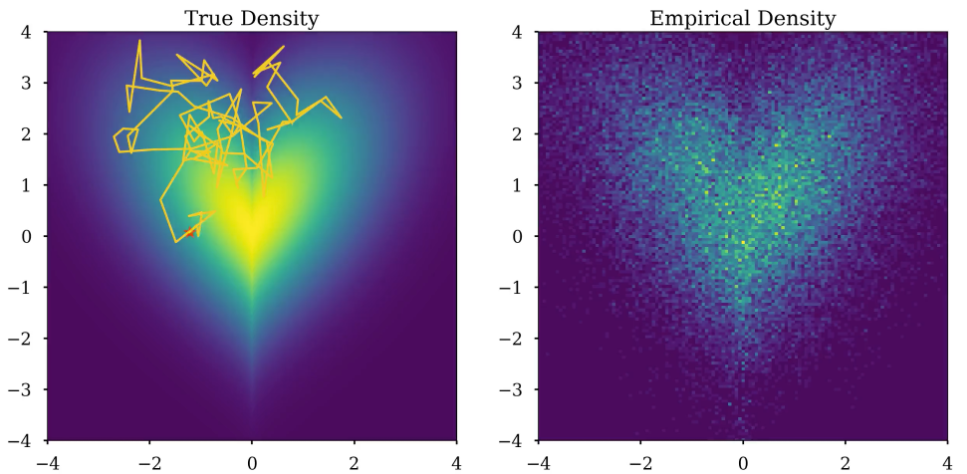
\includegraphics[width=.8\textwidth]{Chapters/figures/langevin.PNG}
    \caption[Application of Langevin Dynamics sampling]{Application of Langevin Dynamics sampling. Figure from\\ https://abdulfatir.com/Langevin-Monte-Carlo/}
\end{figure}
%%%%%%%%%%%%%%%%%%%%%%%%%%%%%%%%%%%%%%%%%%%%%%%%%%%%%%%%%%%%%%%%%%%%%%%%%%%%%%%%%%%%%%%%%%%%%%
\section{Hindrances of a na\"{i}ve applicaton} \label{sec:4.2}
While this general concept looks quite appealing to use as the basis for a generative model, in its na\"{i}ve application it might fail for datasets containing real world data. The authors of \cite{score_1} discuss two hindrances preventing this na\"{i}ve application which both are bypassable by adding random noise to the data. These bypasses also have some consequences on Score Matching and Langevin Dynamics which will be discussed in \hyperref[sec:4.3]{Sec.\,4.3}. It should be noted, however, that the final score-based model (\hyperref[sec:4.4]{Sec.\,4.4}) which we will derive in the following two sections can also be derived from considerations other than those described in this section.
%
\subsection{The manifold hypothesis} \label{sec:4.2.1}
The problems in both \hyperref[sec:4.2.1]{Sec.\,4.2.1} and \hyperref[sec:4.2.2]{Sec.\,4.2.2} originate from a similar source: The data density of a dataset of real world data. The manifold hypothesis states that real world high-dimensional data lies on low-dimensional manifolds embedded within the high-dimensional space which is called the ambient space. To further explain this hypothesis with an example one can imagine a dataset of black and white images, each image being $m\times n$ in size. The ambient space – the space of \textit{all} possible black and white images with that size – has therefore $m\times n$ dimensions. Datasets normally do not contain all possible data of a kind which would make them useless but rather contain data that is very special, e.g. images of cars. As there is some similarity in cars the data in such a dataset is assumed to only cover a small, connected volume in the high dimensional space – a manifold. 

With this hypothesis two problems arise for score-models as they are described above. First, the score $\nabla_{\vec{x}}\log p_{data}(\vec{x})$ is calculated in the whole ambient space, i.e. for all dimensions, not only for the lower dimensions of the manifold. This results in the score being undefined when $\vec{x}$ is confined to such a low dimensional manifold. Second, it was shown in \cite{score_matching_original} that the objective from \hyperref[equ:4.2]{Equ.\,4.2} can only be used for defining a consistent score estimator when the data, the data distribution describes, has the same dimensionality as the whole space.
%
\subsection{Low data density region}\label{sec:4.2.2}
A second problem that arises with the data distribution of a dataset of real world data is that there is just not enough data to fully cover the data distribution. Recall that the data distribution is unknown and describes \textit{all} data of a kind. To make an example, if a model should learn to generate cars, then the data distribution would contain \textit{all} images of cars one can imagine. Certainly we are not able to create a dataset containing images of all cars which in reverse means that the dataset most likely focuses on data that is particularly representative for the data the model should learn.

This has some consequences for score estimation. For data distributions there are regions of high density, where a lot of data is expected. In datasets – as they try to represent the data distribution – most data should appear in this high density regions. But there are also low density regions where little or no data is available. In the car example from above this means that there might be a lot of images of blue or black cars but little or no images of yellow cars. In that regions of low density the score cannot be estimated as there is no data to learn from. In mathematical representation this means that when considering any region $\mathcal{R}\subset\mathbb{R}^d$ in a dataset $\{\vec{x}_i\}_{i=1}^N\overset{i.i.d}{\sim}p_{data}(\vec{x})$ such that $p_{data}(\mathcal{R})\approx0$ the intersection $\{\vec{x}_i\}_{i=1}^N\cap\mathcal{R}$ is often equal to the empty set $\varnothing$. 

%%%%%%%%%%%%%%%%%%%%%%%%%%%%%%%%%%%%%%%%%%%%%%%%%%%%%%%%%%%%%%%%%%%%%%%%%%%%%%%%%%%%%%%%%%%%%%
\section[Introducing noise to the data distribution]{Introducing noise to the data distribution%
    \sectionmark{Introducing noise}} \label{sec:4.3}
\sectionmark{Introducing noise}
To mitigate the hindrances stated in \hyperref[sec:4.2.1]{Sec.\,4.2.1} and \hyperref[sec:4.2.2]{Sec.\,4.2.2} the data is perturbed with random Gaussian noise. For the problem in \hyperref[sec:4.2.1]{Sec.\,4.2.1}, adding small Gaussian noise to the data ensures that the perturbed data distribution has the same dimensionality than the whole space fixing the problem with the inconsistent score estimator. In addition the disturbed data distribution no longer concentrates on a low dimensional manifold so the score is now defined everywhere in ambient space.

The solution to the problem in \hyperref[sec:4.2.2]{Sec.\,4.2.2} is similar but requires large Gaussian noise. This large noise perturbes the data distribution in such a way that low density regions in the original data distribution are filled which makes it possible for the score-models to improve on learning the score in low density regions.

The idea is then to use multiple noise scales with decreasing magnitude to transform the maximum noise-perturbed data distribution via a sequence of lower noise-perturbed data distributions to the true (unnoised) data distribution. This idea provokes several changes for the score-model $s_\theta(\vec{x})$ and the Langevin Dynamics sampling procedure. 
%
\subsection{Noise Conditional Score Networks} \label{sec:4.3.1}
As there is now a sequence of data distributions with decreasing noise, the score-model no longer aims to learn the score of one data distribution but to jointly learn the score of all data distributions. The noise can be thought of as a parameter which is given to the network additionally the data $\vec{x}$. Such a model $s_\theta(\vec{x}, \sigma)$ is called a \textit{Noise Conditional Score Network} (NCSN) \cite{score_1}. In practice when giving the model a value $\vec{x}_\sigma$ from a noisy data distribution $q_{\sigma_i}(\vec{x})\triangleq\int p_{data}(\vec{t})\mathcal{N}(\vec{x}|\vec{t},\sigma_i^2I)d\vec{t}$ the variance $\sigma_i$ of this distribution is given as a parameter to the model so it can learn the difference between various noise scales applied to data $\vec{x}$. The authors of \cite{score_1} choose the noise scales $\{\sigma_i\}_{i=1}^L$ as a positive geometric series, i.e. $\frac{\sigma_1}{\sigma_2}=\dots=\frac{\sigma_{L-1}}{\sigma_L}$ where $\sigma_L$ denotes the smallest noise scale and $\sigma_1$ the largest noise scale. A high $\sigma_1$ was found to be significant for the diversity of the samples \cite{score_2}. However, a high $\sigma_1$ comes with the flaw of high computational expenses of Langevin Dynamics. \cite{score_2} shows that choosing $\sigma_1$ as the maximum Euclidean distance between all pairs of training data points is a good choice. In general, if the score-model is properly trained, then $\forall\sigma\in\{\sigma_i\}_{i=1}^L$ applies $s_\theta(\vec{x}, \sigma)\approx\nabla_{\vec{x}}\log q_\sigma(\vec{x})$, making $s_\theta(\vec{x},\sigma)$ a nearly perfect score estimator on all noise scales. 

To achieve high quality samples the model architecture has to be well adapted to the task of noise-conditional Score Matching. The model the authors of \cite{score_1} use is called NCSN (Noise Conditional Score Network) and is build upon successful model architectures from dense semantic segmentation a.o. U-Net (\hyperref[sec:3.1.2]{Sec.\,3.1.2}). When advancing score-models to continuous noise in \hyperref[sec:4.4]{Sec.\,4.4} the authors of \cite{score_3} introduce an improved model called NCSN++ which is strongly based on the model implementation of \cite{ho2020denoising}.

In order to train a NCSN the objective of noise-conditional Score Matching must be known. The noise distributions get chosen as $q_\sigma(\tilde{\vec{x}}|\vec{x})=\mathcal{N}(\tilde{\vec{x}}|\vec{x},\sigma^2I)$; therefore $\nabla_{\tilde{\vec{x}}}\log q_\sigma(\tilde{\vec{x}}|\vec{x})=-\nicefrac{(\tilde{\vec{x}}-\vec{x})}{\sigma^2}$. For a given $\sigma\in\{\sigma_i\}_{i=1}^L$ the objective can be formulated as a adaption of \hyperref[equ:4.3]{Equ.\,4.3}:
%
\begin{equation} \label{equ:4.8}
    \ell(\theta; \sigma)\triangleq\frac{1}{2}\mathbb{E}_{p_{data}(\vec{x})}\mathbb{E}_{\tilde{\vec{x}}\sim\mathcal{N}(\vec{x},\sigma^2I)}\left[\norm{s_\theta(\tilde{\vec{x}},\sigma)+\frac{\tilde{\vec{x}}-\vec{x}}{\sigma^2}}_2^2\right]
\end{equation}
% 
To get one unified objective \hyperref[equ:4.8]{Equ.\,4.8} is summed for all noise scales $\sigma\in\{\sigma_i\}_{i=1}^L$:
%
\begin{equation} \label{equ:4.9}
    \mathcal{L}(\theta;\{\sigma_i\}_{i=1}^L)\triangleq\frac{1}{L}\sum_{i=1}^L\lambda(\sigma_i)\ell(\theta;\sigma_i)
\end{equation}
%
Here $\lambda(\sigma_i)>0$ is a coefficient function depending on $\sigma_i$. As it is advantageous when the scores of all levels of noise have roughly the same order of magnitude and empirically it is observed that $\norm{s_\theta(\vec{x},\sigma)}_2\propto\nicefrac{1}{\sigma}$ \cite{score_2}, $\lambda(\sigma)$ is chosen to be $\sigma^2$. With that choice the term $\lambda(\sigma_i)\ell(\theta;\sigma_i)$ in \hyperref[equ:4.9]{Equ.\,4.9} is equal to $\sigma^2\ell(\theta;\sigma_i)=\frac{1}{2}\mathbb{E}[\norm{\sigma s_\theta(\tilde{\vec{x}},\sigma)+\frac{\tilde{\vec{x}}-\vec{x}}{\sigma^2}}_2^2]$. Because $\frac{\tilde{\vec{x}}-\vec{x}}{\sigma^2}\sim\mathcal{N}(0, I)$ and $\norm{\sigma s_\theta(\tilde{\vec{x}},\sigma)}\propto1$ we can deduce that the order of magnitude of $\lambda(\sigma)\ell(\theta;\sigma)$ is independent of $\sigma$.
%
\subsection{Annealed Langevin Dynamics} \label{4.3.2}
After introducing noise scales is is clear that also the Langevin Dynamics algorithm has to be adjusted. In \hyperref[sec:4.1.2]{Sec.\,4.1.2} we saw that Langevin Dynamics transforms a sample $\tilde{\vec{x}}_0$ from a prior distribution $\pi(\vec{x})$ to a sample $\tilde{\vec{x}}_T$ from the target data distribution $p_{data}$ by applying $T$ steps of Langevin Dynamics algorithm (\hyperref[equ:4.7]{Equ.\,4.7}). Now the goal remains the same but it is not possible to directly transform the prior distribution to the data distribution because the score-model only knows the scores for certain noise levels. Instead \hyperref[equ:4.7]{Equ.\,4.7} is applied $L$ times in a sequence, once for each transition from one noise distribution $q_{\sigma_i}(\vec{x})$ to another $q_{\sigma_{i+1}}(\vec{x})$. This means, that starting from an initial sample $\tilde{\vec{x}}_0$ from a prior distribution that is perturbed with the maximum noise $\sigma_1$ – i.e. $\pi(\vec{x})\sim q_{\sigma_1}(\vec{x})$ – this sample is then transformed to be a sample of the noise distribution $q_{\sigma_{2}}(\vec{x})$. The procedure is then repeated by using the final sample $\tilde{\vec{x}}_T$ from the last step as the new initial sample $\tilde{\vec{x}}_0$ that is then be transformed to be a sample of the noise distribution $q_{\sigma_{3}}(\vec{x})$. After $L$ of such steps we therefore have a sample of $q_{\sigma_L}(\vec{x})\approx p_{data}(\vec{x})$. The final algorithm can be seen in \hyperref[alg:1]{Alg.\,1}.
%
\begin{algorithm} \label{alg:1}
    \DontPrintSemicolon
    \Require{$\{\sigma_i\}_{i=1}^L,\epsilon,T$}
    Initialize $\tilde{\vec{x}}_0$\;
    \For{$i\leftarrow$ to $L$}{
        $\alpha_i\leftarrow\epsilon\cdot\sigma_i^2/\sigma_L^2$ \Comment*[r]{$\alpha_i$ is the step size}
        \For{$t\leftarrow1$ to $T$}{
            Draw $z_t\sim\mathcal{N}(0,I)$\;
            $\tilde{\vec{x}}_t\leftarrow\tilde{\vec{x}}_{t-1}+\frac{\alpha_i}{2}s_\theta(\tilde{\vec{x}}_{t-1},\sigma_i)+\sqrt{\alpha_i}\vec{z}_t$
        }
        $\tilde{\vec{x}}_0\leftarrow\tilde{\vec{x}}_T$
    }
    \Return{$\tilde{\vec{x}}_T$}
    \caption[Annealed Langevin Dynamics]{\textsc{Annealed Langevin Dynamics} (adapted from \cite{score_1})}
\end{algorithm}

Here $\alpha_i$ denotes the outer step size that is tuned down gradually by $\alpha_i=\epsilon\cdot\sigma_i^2/\sigma_L^2$. Since the noise distributions $\{\sigma_i\}_{i=1}^L$ are perturbed with Gaussian noise the scores encountered during sampling are all well defined. Also, when $\sigma_1$ is sufficiently large there are less low density regions in $q_{\sigma_1}(\vec{x})$, preventing the algorithm to encounter regions where the score has not been learned due to a lack of training data.

With the release of \cite{score_1} the authors found that their \textit{FID (Fréchet inception distance)} \cite{fid} scores – a metric for evaluating the quality of samples – was higher (worse) than state-of-the-art FID scores even though the samples looked better to human eyes. Thereupon \cite{score_4} found that the final sample generated by \hyperref[alg:1]{Alg.\,1} contains some noise which is not visible to the human eye but noticeably decreases the FID score. To solve this problem the authors of \cite{score_4} proposed to add an extra denoising step after the original Annealed Langevin Dynamics which significantly improves FID scores. This improved algorithm can be found in \hyperref[alg:2]{Alg.\,2}.
%
\begin{algorithm} \label{alg:2}
    \DontPrintSemicolon
    \Require{$\{\sigma_i\}_{i=1}^L,\epsilon,T$}
    Initialize $\tilde{\vec{x}}_0$\;
    \For{$i\leftarrow$ to $L$}{
        $\alpha_i\leftarrow\epsilon\cdot\sigma_i^2/\sigma_L^2$\;
        \For{$t\leftarrow1$ to $T$}{
            Draw $z_t\sim\mathcal{N}(0,I)$\;
            $\tilde{\vec{x}}_t\leftarrow\tilde{\vec{x}}_{t-1}+\frac{\alpha_i}{2}s_\theta(\tilde{\vec{x}}_{t-1},\sigma_i)+\sqrt{\alpha_i}\vec{z}_t$
        }
        $\tilde{\vec{x}}_0\leftarrow\tilde{\vec{x}}_T$
    }
    \If{denoise $\tilde{\vec{x}_T}$}{
        \Return{$\tilde{\vec{x}}_T +\sigma^2_Ls_\theta(\tilde{\vec{x}}_T,\sigma_L)$}
    }
    \Else{
        \Return{$\tilde{\vec{x}}_T$}
    }
    
    \caption[Improved Annealed Langevin Dynamics]{\textsc{Improved Annealed Langevin Dynamics} (adapted from \cite{score_1} and \cite{score_4})}
\end{algorithm}
%%%%%%%%%%%%%%%%%%%%%%%%%%%%%%%%%%%%%%%%%%%%%%%%%%%%%%%%%%%%%%%%%%%%%%%%%%%%%%%%%%%%%%%%%%
\section[The way to continuous noise]{The way to continuous noise%
    \sectionmark{Continuous Noise}} \label{sec:4.4}
\sectionmark{Continuous Noise}
In \hyperref[sec:4.2]{Sec.\,4.2} a sequence of discrete noise scales was used to perturb the data distribution. Although this score-model produced first visually appealing samples \cite{score_1}, the training image and sample size of the model was limited to $\sim64\times64$. In \cite{score_2} $5$ techniques were proposed which allowed the authors to attain resolutions up to $256\times256$. Most likely is is possible to scale up this model to even higher resolutions but the authors of \cite{score_3} instead proposed a new model which uses continuous noise: Introducing a continuous noise \cite{score_3} instead of discrete noise scales allowed the authors to reach resolutions up to $1024\times1024$, introduces a mathematically pleasant generalization of different Score-Based Models and creates the possibility for a lot more sampling methods than just Langevin Dynamics.
%
\subsection{Score-Based Generative Modeling with SDEs} \label{sec:4.4.1}
The discrete noise scales $\{\sigma_i\}_{i=1}^L$ are now replaced by a diffusion process $\{\vec{x}(t)\}_{t=0}^T$ indexed by a continuous time variable $t\in[0,T]$ that evolves according to a SDE. For the distribution $p_{data}$ of a dataset of i.i.d samples this means that $\vec{x}(0)\sim p_{data}(\vec{x})$ and $\vec{x}(T)\sim \pi(\vec{x})$ where $\pi(\vec{x})$ is a prior distribution that in \textit{completely independent} of $p_{data}$, e.g a Gaussian distribution with fixed mean and variance. The diffusion process can be modeled by the following (Itô-)SDE:
%
\begin{equation} \label{equ:4.10}
    d\vec{x}=\vec{f}(\vec{x},t)dt+g(t)d\vec{w}
\end{equation}
%
In \hyperref[equ:4.10]{Equ.\,4.10} the vector-valued function $\vec{f}(\cdot,t):\mathbb{R}^d\rightarrow\mathbb{R}^d$ is called the \textit{drift coefficient}, the scalar function $g(\cdot):\mathbb{R}\rightarrow\mathbb{R}$ is called the \textit{diffusion coefficient} and $\vec{w}$ denotes the \textit{Wiener process}. In general $g(\cdot)$ could also be a $d\times d$ matrix but for the ease of presentation a scalar diffusion coefficient is assumed. How to choose the diffusion coefficient and the drift coefficient such that $\vec{x}(t)$ diffuses to $\pi(\vec{x})$ is explained in \hyperref[sec:4.4.4]{Sec.\,4.4.4}.

A remarkable result \cite{ANDERSON} is that such a SDE has a reverse SDE that models a reverse time diffusion process, diffusing a sample $\vec{x}(T)\sim\pi(\vec{x})$ to $p_{data}(\vec{x})$:
%
\begin{equation} \label{equ:4.11}
    d\vec{x}=[\vec{f}(\vec{x},t)-g(t)^2\nabla_{\vec{x}}\log p_t(\vec{x})]dt+g(t)d\vec{\Bar{w}}
\end{equation}
%
Here $dt$ is an infinitesimal timestep backwards in time and $\vec{\Bar{w}}$ is the Wiener process running backwards in time. For the application of this reverse diffusion process it comes very hand that it only depends on the score $\nabla_{\vec{x}}\log p_t(\vec{x})$. So if the score of each noisy distribution $p_t(\vec{x})$ of $\vec{x}(t)$ ($t\in[0, T]$) is known it is possible to sample from $p_{data}$ by solving the reverse SDE.
%
\subsection{Denoising Diffusion Probabilistic Models}
Denoising Diffusion Probabilistic Models (DDPM) \cite{ho2020denoising} are closely related to SMLD (\hyperref[sec:4.3.1]{Sec.\,4.3.1}). They very briefly will be presented here as they can be generalized together with SMLD to continuous NCSN (\hyperref[sec:4.4.3]{Sec.\,4.4.3}, \hyperref[sec:4.4.4]{Sec.\,4.4.4}). DDPMs are trained on Markov chains whose transitions are learned by the model to reverse a diffusion process by reversing the Markov chain. This will especially work if the diffusion consists of small amounts of Gaussian noise \cite{ho2020denoising}. The objective of such a models is given as 
%
\begin{equation} \label{equ:4.12} 
    \theta^*=\underset{\theta}{\arg\min}\,\sum_{i=1}^N(1-\alpha_i)\mathbb{E}_{p_{data}(\vec{x})}\mathbb{E}_{p_{\alpha_i}(\tilde{\vec{x}}|\vec{x})}\left[\norm{s_\theta(\tilde{\vec{x}},i)-\nabla_{\tilde{\vec{x}}}\log p_{\alpha_i}(\tilde{\vec{x}}|\vec{x})}_2^2\right],
\end{equation}
%
where $\alpha_i\triangleq\Pi_{j=1}^i(1-\beta_j)$ and $0<\beta_1<\beta_2,\dots,\beta_N<1$ are positive noise scales. The Markov chain $\{\vec{x}_i\}_{i=0}^N$ is constructed in such a way that the perturbation kernels $p(\vec{x}_i|\vec{x}_{i-1})=\mathcal{N}(\vec{x_i};\sqrt{1-\beta_i}\,\vec{x}_{i-1},\beta_i\vec{I})$. Starting with an initial sample $\tilde{\vec{x}}_N$ and a trained DDPM $s_\theta(\vec{x}_i, \beta_i)$ the following reverse Markov chain can be used to sample from $p_{data}$:
%
\begin{equation} \label{equ:4.13}
    \vec{x}_{i-1}=\frac{1}{\sqrt{1-\beta_i}}(\vec{x}_i+\beta_is_\theta(\vec{x}_i,i))+\sqrt{\beta_i}\vec{z}_i,\quad i=N,N-1,\dots,1
\end{equation}
%
\subsection{Generalizing the Score Matching objective} \label{sec:4.4.3}
Like in the previous sections some adaptions to the objective of Score Matching have to be made. Without further mathematical derivation a continuous generalization of the previous objectives (\hyperref[equ:4.3]{Equ.\,4.3}, \hyperref[equ:4.9]{Equ.\,4.9}, \hyperref[equ:4.12]{Equ.\,4.12}) is given as
%
\begin{equation} \label{equ:4.14}
    \theta^*=\underset{\theta}{\arg\min}\,\mathbb{E}_t\left\{\lambda(t)\mathbb{E}_{\vec{x}(0)}\mathbb{E}_{\vec{x}(t)|\vec{x}(0)}\left[\norm{s_\theta(\vec{x}(t),t)-\nabla_{\vec{x}(t)}\log p_{0t}(\vec{x}(t)|\vec{x}(0))}_2^2\right]\right\}.
\end{equation}
%
$\lambda(t):[0,T]\rightarrow\mathbb{R}_{>0}$ is a positive weighting function. Similarly to the weighting function in \hyperref[equ:4.9]{Equ.\,4.9} it is chosen in a way such that the magnitude of the score is independent of the noise – here characterized by $t$ – which implies a choice of the form $\lambda\propto 1/\mathbb{E}\norm{\nabla_{\vec{x}(t)}\log p_{0t}(\vec{x}(t)|\vec{x}(0))}_2^2$.

Moreover, note the similarities of this objective with the one in \hyperref[equ:4.3]{Equ.\,4.3}. The objective in general is now dependent on $t$ and the discrete noise distributions have been replaced by transition kernels $p_{st}(\vec{x}(t)|\vec{x}(s))$ describing a transition from $\vec{x}(s)$ to $\vec{x}(t)$ where $0\leq s \leq t \leq T$.
%
\subsection{VE and VP SDEs} \label{sec:4.4.4}
In general there is are infinite ways to choose the drift coefficient $\vec{f}(\vec{x}(t),t)$ and the diffusion coefficient $g(t)$ in \hyperref[equ:4.10]{Equ.\,4.10}. Having said that, there are two especially interesting ways to choose $\vec{f}$ and $g$. It is namely that the noise pertubations used in SMLD and DDPM correspond to discretizations of two types of SDEs. With that knowledge the concepts of SMLD and DDPM can be transformed to two different implementations of the continuous noise model.

For SMLD, perturbation kernels of the form $p_{\sigma_i}(\tilde{\vec{x}}|\vec{x})=\mathcal{N}(\tilde{\vec{x}}|\vec{x},\sigma^2\vec{I})$ with $i\in\{1,\dots,N\}$ are deployed. Applying these perturbation kernels in series on a variable $\vec{x}$ can be written as the following Markov chain:
%
\begin{equation} \label{equ:4.15}
    \vec{x}_i=\vec{x}_{i-1}+\sqrt{\sigma_i^2-\sigma_{i-1}^2}\vec{z}_{i-1},
\end{equation}
%
where $\vec{z}_{i-1}\sim\mathcal{N}(\vec{0},\vec{I})$. $\vec{x}_0\sim p_{data}$ and $\sigma_0$ is chosen as $0$. $\vec{x}_i$, $\sigma_i$ and $z_i$ are now reformulated as $\vec{x}(\nicefrac{i}{N})$, $\sigma(\nicefrac{i}{N})$ for $z(\nicefrac{i}{N})$ for $i=1,2,\dots,N$. With $\Delta t=\nicefrac{1}{N}$ and $t\in\{0,\nicefrac{1}{N},\dots,\nicefrac{N-1}{N}\}$ \hyperref[equ:4.15]{Equ.\,4.15} can be rewritten as
%
\begin{equation} \label{equ:4.16}
    \vec{x}(t+\Delta t)=\vec{x}(t)+\sqrt{\sigma^2(t+\Delta t)-\sigma^2(t)}\,\vec{z}(t).
\end{equation}
%
With the assumption $\Delta t \ll 1$ \hyperref[equ:4.16]{Equ.\,4.16} can be approximated as 
%
\begin{equation} \label{equ:4.17}
    \vec{x}(t+\Delta t)=\vec{x}(t)+\sqrt{\frac{d\sigma^2(t)}{dt}\Delta t}\,\vec{z}(t),
\end{equation}
%
and in the limit of $\Delta t\rightarrow 0$ (continuous), \hyperref[equ:4.17]{Equ.\,4.17} converges to 
%
\begin{equation} \label{equ:4.18}
    d\vec{x}=\sqrt{\frac{d\sigma^2(t)}{dt}}\,d\vec{w}.
\end{equation}
%
This SDE is called the \textit{VE SDE} and describes the continuous stochastic process $\{\vec{x}(t)\}_{t=0}^1$ of the former discrete Markov chain $\{\vec{x}_i\}_{i=1}^N$. In the representation of \hyperref[equ:4.10]{Equ.\,4.10} this means that $\vec{f}(\vec{x},t)=0$ and $g(t)=\sqrt{\frac{d\sigma^2(t)}{dt}}$.

Using the same procedure also the perturbation kernels of DDPM can be transformed to a continuous stochastic process leading to
%
\begin{equation} \label{equ:4.19}
    d\vec{x}=-\frac{1}{2}\beta(t)\vec{x}\,dt+\sqrt{\beta(t)}\,d\vec{w},
\end{equation}
%
which is called the \textit{VP SDE}. The names VE and VP originate from the observations that the VE SDE always gives a process with \textbf{E}xploding \textbf{V}ariance whist the VP SDE yields a process with bounded variance, therefore \textbf{P}reserving the initial \textbf{V}ariance. The variance of the SDEs are given as the variance of their perturbation kernels $p_{0t}(\vec{x}(t)|\vec{x}(0))$, which are $[\sigma^2(t)-\sigma^2(0)]\vec{I}$ for the VE SDE and $\vec{I}-\vec{I}\exp{-\int_0^t\beta(s)ds}$ for the VP SDE. As the VE SDE is better suited to produce high resolution images \cite{score_3} and is easier to implement we exclusively use the VE SDE in our experiments.

\subsection{Sampling via the Reverse SDE}
As mentioned in \hyperref[sec:4.4.1]{Sec.\,4.4.1}, samples of $p_{data}$ can be generated by solving the reverse SDE. In order to do so the scores $\nabla_{\vec{x}}\log p_t(\vec{x})$ are needed which are provided by the trained score-model $s_\theta(\vec{x}(t),t)$. In theory, to solve the reverse SDE any kind of numerical SDE solver can be used. In practice, however, it was determined that most off-the-shelf SDE solvers are ill-suited for generative modeling \cite{gotta_go_fast}. These off-the-shelf SDE solvers often exhibit divergence, slow data generation and worse quality than than the specialized SDE solvers proposed beneath.

\subsubsection{Predictor Corrector samplers}
The first sampling strategy - which is also the one we use for all experiments – consists of a predictor and a corrector. This category of samples is therefore is called \textit{Predictor-Corrector Samplers} \cite{score_3}. The sampler works in such a way that the predictor gives an estimate of the sample at the next step and the corrector corrects this estimated sample. The idea to use a combination of a predictor and a corrector instead solely using a SDE solver comes from the realization that we have additional information in the reverse SDE (\hyperref[equ:4.11]{Equ.\,4.11}): the score. We have seen in \hyperref[sec:4.3.2]{Sec.\,4.3.2} that the score can be used to sample from $p_{data}$, so we know how to process this extra information which is normally not available when solving arbitrary SDEs. In the implementation a variation of Langevin Dynamics samplers plays the role of the corrector and and a numerical SDE solver plays the role of the predictor.

The authors of \cite{score_3} propose to use the \textit{Euler-Maruyama Method} as the SDE solver which is a very simple method to numerically solve SDEs and is based on the well known Euler method for solving ordinary differential equations (ODEs). For a general SDE (\hyperref[equ:4.10]{Equ.\,4.10}) the Euler-Maruyama method computes the evolution of $\vec{x}$ as the following recursive formula:
%
\begin{equation} \label{equ:4.20}
    \vec{x}_i=\vec{x}_{i-1}+\tau\vec{f}(\vec{x}_{i-1}, t_{i-1})+g(\vec{x}_{i-1}, t_{i-1})\vec{z_{i-1}},
\end{equation}
%
where $\tau$ is the step size defined as $\tau=\frac{T}{i}$, $\vec{z}_{i-1}\sim\mathcal{N}(\vec{0},\vec{I})$, $i=0,\dots,N$ and $0=t_0<t_1<\dots<t_n=T$ is the discretization of time $t$. We have seen such a discretization of a SDE before in \hyperref[equ:4.15]{Equ.\,4.15}. From this realization follow two points: First, the discretization in \hyperref[equ:4.15]{Equ.\,4.15} is called Euler-Maruyama discretization and second, the Euler-Maruyama discretization is a Markov chain.

The full predictor-corrector algorithm using Langevin Dynamics and the Euler-Maruyama method can be seen in \hyperref[alg:3]{Alg.\,3}. In this algorithm $N$ denotes the number of sampling steps and $snr$ is the signal-to-noise-ratio which adjusts the radio between the scores and the noise. $snr$ has a large effect on sampling quality and is experimentally chosen to be between $\sim0.15$ and $\sim0.075$ depending on the sampling resolution. 
%
\begin{algorithm} \label{alg:3}
    \DontPrintSemicolon
    \Require{$N, snr$}
    Initialize $\tilde{\vec{x}}_0$\;
    \For{$i\leftarrow1$ to $N$}{
        Draw $z_i\sim\mathcal{N}(0,I)$ \Comment*[r]{Langevin Dynamics}
        $\epsilon_{i-1}\leftarrow\left[\frac{snr\cdot\norm{\vec{z}_{i-1}}}{\norm{s_\theta(\tilde{\vec{x}}_{t_{i-1}},t_{i-1})}}\right]^2$\;
        $\tilde{\vec{x}}_{langevin}\leftarrow\tilde{\vec{x}}_{i-1}+2\epsilon_{i-1} \,s_\theta(\tilde{\vec{x}}_{i-1},t_{i-1})+\sqrt{2\epsilon_{i-1}}\,\vec{z}_{i-1}$\;
        \;
        Draw $z_i\sim\mathcal{N}(0,I)$ \Comment*[r]{Euler-Maruyama}
        $\Delta t_i\leftarrow t_{i-1}-t_i$\;
        $\tilde{\vec{x}}_i\leftarrow\tilde{\vec{x}}_{langevin}+ \vec{f}(\tilde{\vec{x}}_{langevin}, t_{i-1})\cdot \Delta t_{i}+g(\tilde{\vec{x}}_{i-1}, t_{i-1})\cdot\sqrt{\Delta t_i}\,\vec{z}_{i-1}$
    }
    \Return{$\tilde{\vec{x}}_N$}

    
    \caption[Predictor-Corrector Sampler]{\textsc{Predictor-Corrector Sampler}}
\end{algorithm}
%
\subsubsection{Probability Flow ODE sampler}
%
This sampling strategy is based upon the mathematical finding that every diffusion process has a corresponding \textit{deterministic process} which is governed by the following \textit{ODE}:
%
\begin{equation} \label{equ:4.21}
    d\vec{x}=\left[\vec{f}(\vec{x},t)-\frac{1}{2}g(t)^2\nabla_{\vec{x}}\log p_t(\vec{x})\right]dt
\end{equation}
%
Deterministic in this sense means that the trajectories of the process are not affected by some kind of randomness but rather can be predicted beforehand. This special ODE which needs the score in order to be determined from the SDE shares the same probability densities $\{p_t(\vec{x})\}_{t=0}^T$ as the SDE. 

An advantage is that the ODE can be solved with numerical \textbf{O}DE solvers which are normally a lot faster than numerical SDE solvers. Nevertheless we do not use this sampling technique because it produces samples of worse quality \cite{score_3} and the other advantages of solving this ODE do not apply for our purpose of use.
%
\subsubsection{Other sampling methods}
%
There were also other sampling methods proposed of which we want to name a few. \textit{Reverse Diffusion Samplers} were proposed in \cite{score_3} together with Predictor-Corrector samplers and Probability Flow samples and are a kind of numerical SDE solvers which discretize the reverse SDE in the same way the forward SDE is discretized.

A promising sampler was proposed as a result of an in-depth sampler analysis and a lot of finetuning in \cite{gotta_go_fast}. These samplers are non-general-purpose SDE solvers which means they are specially tailored to solve the SDE in \hyperref[equ:4.10]{Equ.\,4.10}. This results in sampling speeds $2-10$ times higher than all other mentioned samplers and also in higher sampling quality. However, we leave the exploration of this sampler in context of our work to future research.

%%%%%%%%%%%%%%%%%%%%%%%%%%%%%%%%%%%%%%%%%%%%%%%%%%%%%%%%%%%%%%%%%%%%%%%%%%%%%
\section{Controllable Generation} \label{sec:4.5}
Controllable Generation is the modulation of the generation process. Popular controllable generation tasks include inpainting, colorization, class conditional generation or generation conditioned on semantic maps. For continuous-noise Score-Based Generative Models (\hyperref[sec:4.4]{Sec.\,4.4}), controllable generation can be achieved in an advantageous way. Instead of re-training the model for each controllable generation task, additional information can be used for SGMs during the sampling process to model the controllable generation task.

Basically this means that when we have a trained score-model $s_\theta(\vec{x}, \sigma)$, it is not only possible to sample from $p_{data}(\vec{x}(0))$ but also from $p_{data}(\vec{x}(0)|\vec{y})$ if $p_t(\vec{y}|\vec{x}(t))$ is known. Here $p_{data}(\vec{x}(0)|\vec{y})$ is the data distribution of images with zero noise which fulfill the condition $\vec{y}$ and $p_t(\vec{y}|\vec{x}(t))$ is a probability density function for $\vec{x}(t)$ fulfilling the condition $\vec{y}$ at timestep $t$.

Starting with $p_T(\vec{x}(T)|\vec{y})$ it is possible to solve the following conditional reverse SDE to sample from $p_{data}(\vec{x}(0)|\vec{y})$:
%
\begin{equation} \label{equ:4.22}
    d\vec{x}=\{\vec{f}(\vec{x},t)-g(t)^2[\nabla_{\vec{x}}\log p_t(\vec{x})+\nabla_{\vec{x}}\log p_t(\vec{y}|\vec{x})]\}dt+g(t)d\bar{\vec{w}}.
\end{equation}
%
For class-conditional or semantic map-based generation, the consequence is that a second model is needed to solve the reverse SDE. In \hyperref[equ:4.22]{Equ.\,4.22} the score-model is responsible for the unconditional score $\nabla_{\vec{x}}\log p_t(\vec{x})$, while a second, independently trained model is responsible for the conditional scores $\nabla_{\vec{x}}\log p_t(\vec{y}|\vec{x})$. What seems very mathematical at first is actually very easy to implement.
%
\begin{enumerate}
    \item Train the continuous-noise score-model $s_\theta(\vec{x},\sigma)$ on a dataset of choice.
    \item Train a second model conditioned on the same noise which is able to output $\vec{y}$ from $\vec{x}(t)$. For semantic image synthesis, this would mean training a noise-conditional semantic segmentation network $p_\theta(\vec{x}, \sigma)$ (\hyperref[sec:3.1]{Sec.\,3.1}) with noisy images $\vec{x}(t)$ where the semantic map used for error computation is $\vec{y}$ of the original image $\vec{x}(0)$.
    \item During training add the scores of the score-model to the scores of the noise-conditional segmentation network. To obtain scores from the segmentation network, compare the prediction $\vec{y}(t)$ from the sample $\vec{x}(t)$ at the current sampling step $t$ to the target segmentation map $\vec{y}$ and compute the gradients that would make $\vec{y}(t)$ look more like $\vec{y}$.
\end{enumerate}

